\documentclass{beamer}
\usepackage[utf8]{inputenc}

\usepackage{minted}
\usepackage{pgf}
\usepackage{tikz}
\usepackage{upquote}
\usepackage{hyperref}
\usepackage{graphicx}
\usetikzlibrary{arrows,automata,positioning}

\setbeamertemplate{footline}[frame number]
\setbeamertemplate{navigation symbols}{}

\title{Verified Time Balancing of Security Protocols}
\author{Donovan Crichton}
\date{January 2019}

\begin{document}
 
\frame{\titlepage}

\begin{frame}[fragile]
  \frametitle{Motivation}
  \begin{itemize}
    \item ASD manually verifies vendor code with containing 
          cryptographic processes.
    \item Formal Methods: A mathematically based approach to the
            specification and verification of software.
    \item Can we reduce some of the resources ASD spends on 
            manual verification by replacing with automatic 
            verification?
    \item A case study, also work towards more secure protocols.
  \end{itemize}
\end{frame}

\begin{frame}[fragile]
  \frametitle{Formally Verifying a Time Balanced Security Protocol}
  \begin{itemize}
    \item Attackers can gain information from message timing.
    \item Can we model this invariant? Naively all operations 
          have the same running time.
    \item Can we ensure that assumptions on this model hold for the
            implementation?
  \end{itemize}
\end{frame}

\begin{frame}[fragile]
  \frametitle{The ZRTP Protocol}
  \begin{itemize}
    \item Initially started with ZRTP.
    \item ZRTP is complex and makes many decisions.
    \item Simplified version that contains just enough detail to 
            allow us to attempt to prove some interesting things!
  \end{itemize}
\end{frame}

\begin{frame}[fragile]
  \frametitle{The Simplified Protocol}
    \begin{itemize}
      \item Commit messages contain hashes of 256 bit random nonce.
      \item Diffie-Hellman key exchange contains modulo arithmetic.
      \item How can we formally guarantee the timing of operations?
    \end{itemize}
\end{frame}

\begin{frame}[fragile]
  \frametitle{Approach}
  \begin{itemize}
    \item We can use the notion of propositions as types.
    \item Dependently typed functional programming languages
            also act as theorem provers for a higher-order
                  constructive logic.
    \item We can model this protocol in such a language, Idris.
    \item We can express proofs about properties of the protocol.
  \end{itemize}
\end{frame}

\begin{frame}[fragile]
  \frametitle{Quick Background 1 - Currying}
  All functions treated as taking a single argument. \\ \\
  $f : \mathbb{N} \rightarrow \mathbb{N} \rightarrow \mathbb{N}$ \\
  $f = + $ \\ \\
  Applying an argument to a multi argument function returns the 
    rest of the function! (Arrow associates to the right)\\ \\
  $f(2) : \mathbb{N} \rightarrow \mathbb{N}$ \\
  $f(2) = 2 + $ \\ \\
  Finally all arguments are applied. \\ \\
  $f(2, 3) : \mathbb{N}$ \\
  $f(2, 3) = 2 + 3 = 5 $
\end{frame}

\begin{frame}[fragile]
  \frametitle{Quick Background 2 - Propositions as Types}
     \begin{table}[h!]
    \begin{tabular}{c|c|c|c}
    \textbf{Logic Term} & \textbf{Logic Symbol} & 
    \textbf{Idris Symbol} & \textbf{Idris Type} \\
    \hline
      Implication & p $\Rightarrow$ q & p \mintinline{haskell}{->} q
      & Function \\
      Conjunction & p $\land$ q & \mintinline{haskell}{(p, q)} 
      & Pair / Tuple \\
      Disjunction & p $\lor$ q & \mintinline{haskell}{Either p q}
      & Tagged Union\\
      Negation & $\lnot$ p & \mintinline{haskell}{p -> Void} &
      Void Type \\
      IFF/Eq & p $\equiv$ q, p $\iff$ q & 
        \mintinline{haskell}{(p -> q, q -> p)} 
      & Pair Arrows \\
      Universal & $\forall$ x. P x & 
      \mintinline{haskell}{p -> Type} & $\Pi$ Type \\
      Existential & $\exists$ x. P x 
      & \mintinline{haskell}{(x ** P x)} & $\Sigma$ Type \\
      \hline
       & & \mintinline{haskell}{p = q} & Type Equality
    \end{tabular}
  \end{table}
\end{frame}

\begin{frame}[fragile]
  \frametitle{Quick Background 3 - Idris Syntax and Values as Types}
  Building a vector type in Idris: 
  \begin{minted}{haskell}
    data Vec : Nat -> Type -> Type where
      Nil  : Vec 0 a
      (::) : (x : a) -> Vec n a -> Vec (n + 1) a
  \end{minted}
  We can parameterise types over values to capture invariants in 
  the model.
  \begin{minted}{haskell}
    append : Vec n a -> Vec m a -> Vec (n + m) a
    append Nil ys = ys
    append (x :: xs) ys = x :: append xs ys 
  \end{minted}
\end{frame}

\begin{frame}[fragile]
  \frametitle{Building a type of Prg n}
  \begin{table}[h!]
  \begin{tabular}{c|c|c|c}
  Statement & Continuation & Result & Description \\
  \hline 
  Halt & Prg 1 & Prg 1 & Terminate \\
  AssC & Prg k & Prg (k + 1) & Asn constant. \\
  AssV & Prg k & Prg (k + 1) & Asn variable. \\
  UnOp & Prg k & Prg (k + 1) & Asn result of unary op. \\
  BinOP & Prg k & Prg (k + 1) & Asn result of binary op. \\
  Do & Prg k & Prg (m * n + k) & Run Prg m, n times. \\
  Cond & Prg k & Prg (n + k) & Branch on Prg n. \\
  \end{tabular} 
  \end{table}
  Conditionals require both branches to be Prg n. Ensuring
  That all branches of the program are correct by construction.
\end{frame}

\begin{frame}[fragile]
  \frametitle{What about more expressive time parameters?}
  \begin{minted}{haskell}
  f : Value -> Value -> Nat
  f = --some complex function to calculate the number of
      --computation steps for each input to mod.
  
  data Prg : Nat -> Type where
    Mod : {k : Nat} -> (cont : Prg k) -> (x : Value) ->
          (y : Value) -> Prg ((f x y) + k)
  \end{minted}
\end{frame}

\begin{frame}[fragile]
  \frametitle{Elaboration and Compilation of a Correct Core}
  %diagram on how a small correct core can be both elaborated and 
  %compiled
  %for compiled can be mapped to a specific chipset achitecture
  \begin{minipage}[c]{5cm}
  \begin{center}
    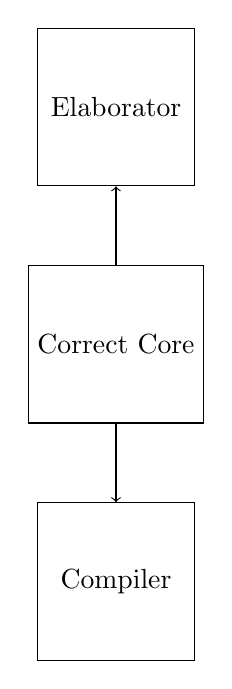
\begin{tikzpicture}
      \node[shape=rectangle, draw=black, minimum size = 2cm] (Elab) 
           {Elaborator} ;
      \node[shape=rectangle, draw=black, minimum size = 2cm] (Prg) 
           [below = 1cm of Elab] {Correct Core};
      \node[shape=rectangle, draw=black, minimum size = 2cm] (Comp) 
           [below = 1cm of Prg] {Compiler};

      \path [->] (Prg) edge node {} (Elab);
      \path [->] (Prg) edge node {} (Comp);
  \end{tikzpicture}
  \end{center}
  \end{minipage}
  \begin{minipage}[c]{\textwidth-6cm}
  \begin{itemize}
    \item The small, correct core language can be elaborated to
          a more full-featured language.
    \item The size of the core language makes the burden of proofs
          much lighter.
    \item The compiler can map the core language expressions down
          to something more real world (e.g C, assembler).
  \end{itemize}
  \end{minipage}
\end{frame}

\begin{frame}[fragile]
  \frametitle{Contributions}
  \begin{itemize}
    \item Formal description of a simplified protocol.
    \item Prg: A small language parameterised over computational 
          time
    \item Some small proofs of Prg correctness.
  \end{itemize}
\end{frame}

\begin{frame}[fragile]
  \frametitle{Further Work}
  \begin{itemize}
    \item Implement the simplified protocol in Prg.
    \item Modulo arithmetic cases.
    \item Relax some of the (many) assumptions.
    \item Investigate elaboration and compilation with regard to 
          invariants.
  \end{itemize}
\end{frame}
\end{document}
